\section{边界以及环境设置}

\subsection{环境压力(背景压力)}

\begin{frame}
    \begin{figure}[H]
        \centering
        \subfigure[低压区]{
            \includegraphics[width=0.6\textwidth]{images/low_pressure_field.png}
        }\\
        \subfigure[局部粒子打穿流场]{
            \includegraphics[width=0.6\textwidth]{images/emit_like_bullet.png}
        }
    \end{figure}
\end{frame}

\begin{frame}
    增加背景压力这件事情是不可行的,
    或者说在液柱垮塌问题中是不可行的。
    回顾压力项的核插值格式:
    \begin{equation}
        \left(\frac{1}{\rho}\nabla p\right)_i
        =
        \sum_j m_j
        \left(\frac{p_i}{\rho_i^2}+\frac{p_j}{\rho_j^2}\right)
        \nabla W_{ij}
    \end{equation}
    如果将背景压力 $p_0$ 加入到这个式子中,
    那么上述压力项就变成了:
    \begin{equation}
        \left(\frac{1}{\rho}\nabla p\right)_i
        =
        \sum_j m_j
        \left(\frac{p_i}{\rho_i^2}+\frac{p_j}{\rho_j^2}\right)
        \nabla W_{ij}
        +
        \sum_j m_j
        \left(\frac{p_0}{\rho_i^2}+\frac{p_0}{\rho_j^2}\right)
        \nabla W_{ij}
    \end{equation}
    \begin{figure}[H]
        \centering
        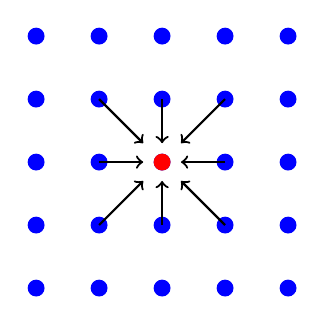
\begin{tikzpicture}
            % draw 5*5 particles
            \foreach \x in {0,1,2,3,4}
            \foreach \y in {0,1,2,3,4}
            {
                \filldraw[blue] (0.8*\x,0.8*\y) circle (0.1);
            }
            % filldraw the center particle as red
            \filldraw[red] (0.8*2,0.8*2) circle (0.1);
            % draw arrow towards the center particle from neighbour particles
            \foreach \x in {1,3}
            \foreach \y in {1,3}
            {
                \draw[->,thick] (0.8*\x,0.8*\y) -- ({0.8*\x + 0.7*0.8*(2-\x)}, {0.8*\y + 0.7*0.8*(2-\y)});
            }
            % draw arrow towards the center particle from neighbour particles up, down, left, right
            \foreach \x in {1,3}
            {
                \draw[->,thick] (0.8*\x,0.8*2) -- ({0.8*\x + 0.7*0.8*(2-\x)}, {0.8*2});
                \draw[->,thick] (0.8*2,0.8*\x) -- ({0.8*2}, {0.8*\x + 0.7*0.8*(2-\x)});
            }
        \end{tikzpicture}
    \end{figure}
\end{frame}

\begin{frame}
    如前图所述,
    当粒子致密的时候,
    会有大量的粒子向中心粒子施加压力,
    靠着足够多的邻域粒子产生的统计效应,
    背景压力会在这种情况下被互相抵消。
    反之,对于多相流问题,
    平白无故地增加背景压力会导致自由表面处背景压强项缺失,
    从而导致粒子的不稳定运动。
    \begin{figure}[H]
        \centering
        \begin{tikzpicture}
            % draw 5*5 particles
            \foreach \x in {0,1,2}
            \foreach \y in {0,1,2,3,4}
            {
                \filldraw[blue] (0.8*\x,0.8*\y) circle (0.1);
            }
            % filldraw the center particle as red
            \filldraw[red] (0.8*2,0.8*2) circle (0.1);
            % draw arrow towards the center particle from neighbour particles
            \foreach \x in {1,3}
            \foreach \y in {1,3}
            {
                \draw[->,thick] (0.8*\x,0.8*\y) -- ({0.8*\x + 0.7*0.8*(2-\x)}, {0.8*\y + 0.7*0.8*(2-\y)});
            }
            % draw arrow towards the center particle from neighbour particles up, down, left, right
            \foreach \x in {1,3}
            {
                \draw[->,thick] (0.8*\x,0.8*2) -- ({0.8*\x + 0.7*0.8*(2-\x)}, {0.8*2});
                \draw[->,thick] (0.8*2,0.8*\x) -- ({0.8*2}, {0.8*\x + 0.7*0.8*(2-\x)});
            }
            \foreach \x in {3,4}
            \foreach \y in {0,1,2,3,4}
            {
                \filldraw[gray] (0.8*\x,0.8*\y) circle (0.1);
            }
            \node[blue] at (-0.5,0.8*2) {水体};
            \node[gray] at (4,0.8*2) {气体};
        \end{tikzpicture}
    \end{figure}
    因此想要增加背景压力,
    正确的做法应该是同时增加气体相的粒子,
    让气体相的粒子在自由表面处产生压力,
    参与进整个流场的压力计算中。
    简言之,
    流域致密的时候可以加背景压力(但也不宜加太多),
    流域稀疏,有多相时,需要增加流相以平衡背景压力。
\end{frame}

\begin{frame}
    一种可能的修正方式是用 Monaghan 的方法,
    在压力项中添加一个斥力:
    \begin{equation}
        \vec{f}_i^p = 
        -\sum_j 
        m_j 
        \left(
            \frac{p_i}{\rho_i^2} + \frac{p_j}{\rho_j^2} + R_{ij}
        \right)\nabla W_{ij}
    \end{equation}
    $R_{ij}$ ($\Delta p$ 为初始粒子间距):
    \begin{equation}
        R_{ij} = 
        0.01
        \left(
            \frac{|p_i|}{\rho_i^2} + \frac{|p_j|}{\rho_j^2}
        \right)
        \frac{W(r_{ij}, h)}{W(\Delta p, h)}
    \end{equation}
    因为核函数是一个“高耸”的函数,因此在 $r_{ij}=\Delta p$ 时,
    压力项仅多了有限的 1\%,而在两粒子很靠近 $r_{ij}\to 0$ 时,
    该斥力项会迅速增大,从而避免了粒子的堆积。
    在实践中,该方法可以很好的解决粒子堆积造成的负压爆炸的问题, 
\end{frame}

\subsection{壁面力}

\begin{frame}
    经过前述描述,
    我们知道了背景压力的作用,
    因为壁面也是用粒子来描述实现的,
    我们可以将壁面力分为三部分:
    \begin{itemize}
        \item 壁面强制力,这部分采用的 Monaghan 的方法,本质上借鉴了接触力学中的概念。
        \item 壁面环境压力,该项仅在流体致密的问题中起作用,对于自由表面问题,不用加入该项。
        \item 壁面粘性*,这部分的引入问题比较大,我会在后续的算例中展示结果与曲线对比。
    \end{itemize}
    \begin{figure}[H]
        \centering
        \begin{tikzpicture}
            \draw[->,thick] (-0.1, 0) -- (3,0);
            \draw[->,thick] (0, -0.1) -- (0,3);
            % draw 1/x 
            \draw[domain=0.3:3,smooth,variable=\x,blue,thick=3] plot ({\x},{1/\x-1/3});
            \node at (3,1.5) {壁面强制力 $0.01\frac{c^2}{h}f(x_\perp)$};
        \end{tikzpicture}
    \end{figure}
\end{frame}

\begin{frame}
    壁面粘性在目前的算例中是存在问题的,
    这里给出一个简单的示意图:
    \begin{figure}[H]
        \begin{tikzpicture}
            \draw[-, thick] (0,0) -- (5,0);
            \node at (-0.5, 0) {壁面};
            \draw[gray] (2,0)--(2,-1)--(3,-1)--(3,0);
            \filldraw[gray] (2.5,-0.5) circle (0.1);
            \draw[blue] (2,0)--(2,1)--(3,1)--(3,0);
            \filldraw[blue] (2.5,0.5) circle (0.1);

            \node[gray] at (2.5, -1.5) {壁面粒子};
            \node[blue] at (2.5, 1.5) {流体粒子};

            \node at (7, 0) {$\vec{v}=0$:理想无滑移边界};
            \node[gray] at (7, -1) {$\vec{v}=0$:按零速度粒子处理的粘性边界};

            % denote wall boundary and wall particle's position -dr/2
            % use } to denote the -dr/2
            \draw[->,thick,red] (3.1,0) -- (3.1,-0.5) node[below] {$-\frac{\Delta p}{2}$};
            
            \draw[dashed] (0.5, 0.5) -- (0.5,-0.5) -- (1.5,-0.5) -- (1.5,0.5) -- (0.5,0.5);
            \filldraw (1,0) circle (0.1);
        \end{tikzpicture}
    \end{figure}
    如果将壁面粒子视作一般的速度为零的水体粒子纳入粘性计算,
    那其实并不能很好的描述壁面无滑移的情况。
    因为粒子客观存在体积,
    进而壁面粒子被埋入墙体 $\frac{\Delta p}{2}$ 的位置,
    真正速度为零的位置被深埋了一段距离。
    另一方面,
    流体粒子因为壁面强制力的原因,
    无法侵入壁面 $\frac{\Delta p}{2}$ 的位置,
    因此其质心始终存在速度,
    不可能贴在墙壁上不运动。

    后续算例的粘性,*会展示将壁面粒子抬高和不抬高 $\frac{\Delta p}{2}$ 的结果对比。
\end{frame}